\chapter{La relative diversité de la représentation des dommages}
\label{chapter:litrev}
\newrefsegment

\PEEL{Les manières de représenter les dommages du changement climatique varient selon leur niveau de désaggrégation, le type de modèle utilisé (simulation / optimisation), leur calibration et les phénomènes qu'elles prennent en compte. }{Nordhaus et Stern se disputent sur la valeur du taux d'actualisation (avec pourtant les mêmes modèles). Le SCC est calculé aux US alors que les dommages ne sont pas pris en compte dans les modèles de l'IIASA database. Il y a une forte utilisation des indicateurs économiques. }{Ces différents duels montrent la diversité de choix possibles offerts aux modélisateur.ices.}{Répondre à ces questions est un choix important, qui dépasse le pure cadre technique pour rejoindre la dimension éthique.}


\chapterabstract{Les fonctions de dommage permettent de modéliser les impacts du changement climatique sur d'autres parties du modèle. Elles peuvent varient par leur existence, forme, calibration ou par les paramètres ou secteurs qu'elles prennent en compte. Pourtant, un changement dans ces fonctions peut radicalement faire changer le fonctionnement d'un modèle, et ainsi les résultats et les conclusions qu'on en tire. Cette partie s'intéresse donc aux différentes fonctions de dommage qui existent dans la littérature.}

%%Accroche
Les modèles intégrés sont ainsi derrière de nombreuses publications qui informent le débat public : rapports du GIEC, Stern Review, revue du coût social du carbone. Ils ont donc un rôle de premier plan dans la prise de décisions sur les questions climatiques, sur les options qu'ils estiment possibles ainsi que sur les conséquences anticipées de telle ou telle action. Un élément clé de cette modélisation est la prise en compte des impacts climatiques. 


%%Définition des termes

%%Rappel du sujet
Les différentes formes de fonction de dommage dans les modèles intégrés

%%Problématique
Quelles sont les fonctions de dommages utilisées dans les modèles intégrés ? Et, plus précisement, quels modèles utilisent des fonctions de dommage ? Quels phénomènes sont représentés ? Quelles variables entrent en compte, et comment sont-elles paramétrisées ? 

%% Annonce du plan
Dans une première partie, nous détaillerons la méthodologie utilisée pour obtenir la base de donnée des fonctions de dommage. Dans une seconde partie, nous la décrirons avec différentes statistiques descriptives. Enfin, nous aborderons trois points critiques des fonctions de dommage : leur forme; leurs paramètres; et la calibration. 

\begin{methodbox}[Revue de la littérature]
Pour obtenir une base de données des différentes fonctions de dommage, nous avons cherché à fusionner plusieurs sources de données. D'abord, l'IAM Consortium publie sur son site internet les documentations de nombreux modèles intégrés, sous la forme d'un wiki. Ces fiches sont rédigées par les équipes des modèles - ce qui permet d'avoir une source primaire sur les informations concernant les modèles - mais sont souvent incomplètes. En revanches, des "cartes", qui détaillent les principales caractéristiques de chaque modèle, sont également disponibles. Ce sont principalement celles-ci qui sont utilisées dans la base de données. Une autre source de données est le fichier des scénarios utilisés par le GIEC. Celui-ci permet d'avoir des informations sur chacun des scénarios soumis pour l'AR6, et d'avoir accès à de nombreuses informations : modèle utilisé, vetted ou non, impacts climatiques pris en compte ou non. A ces différentes sources, on ajoute manuellement des modèles, basée sur une lecture aléatoire de la littérature. Ils comprennenent notablement les modèles utilisés par l'agence interagence du coût social du carbone, ceux cités par Souffron et Jacques, ceux utilisés par les SSP, ainsi que d'autres modèles intégrés trouvés par littérature interposée. 
Le monde de la modélisation est très vaste, les modèles souvent compliqués à comprendre et parfois peu transparents. Ainsi, il a toujours été préféré de se baser sur des sources explicites. Bien qu'un véritable effort pour chercher à avoir une vision sur le plus de modèles possibles, cette étude ne peut pas être considérée comme un recensement exhaustif des modèles intégrés ni de leurs fonctions de dommage. \\ \gls{latex}

Une fois cette première liste de modèles obtenue, un premier tri est effectué entre ceux qui intègrent une fonction de dommage et ceux qui n'en intégrent pas. On considére ici les fonctions de dommages explicitement définies telles quelles, bien que d'autres fonctions puissent in fine avoir un comportement similaire. Ainsi, pour certaines, on a une connaissance explicite : par exemple, les fiches de l'IAMC comportent une case sur les impacts modélisés. Pour les autres, on considère qu'elles n'ont pas de fonction de dommage si les termes "damage function" ou "damage" ne sont pas présents dans leur documentation ou les publications associées, et s'il n'est pas fait mention de fonctions de dommage dans d'autres sources. \\

Pour chaque modèle incluant des fonctions de dommage, on cherche dans sa documentation la description de ces fonctions de dommage. La plupart du temps, celle-ci comporte une équation et les variables associées. Un script Chat-GPT est alors utilisé sur la partie du document qui est décrit la fonction de dommage. Celui-ci interprète et met en forme (sous la forme d'un tableau CSV) toutes les variables présentes dans cette fonction. Elles sont alors contrôlées visuellement. Cette étape est repétée pour chaque fonction de dommage. Une fois les variables de chaque fonction de dommage d'un modèle identifiées, ce fichier est téléversé dans la base de données, à l'aide du logiciel Airtable, dans la table 'Variable'. \\

Une fois les variables insérées dans leur table, les fonctions de dommage sont incluses dans la table 'Damage functions'. Chaque fonction est assortie à un nom, soit celui-donné dans la publication, soit choisi selon le contexte. Sont également ajoutés le nom du modèle, le numéro de l'équation, l'annotation zotero et le DOI de la publication, afin de pouvoir retrouver rapidement la fonction de dommage. Sont alors ajoutés d'une part les variables qui viennent en entrées de l'équation, et la variable qui sur laquelle l'équation agit. \\

Enfin, une autre table est ajoutée : celle des risques identifiés par le GIEC. Ceux-ci sont issus du rapport de synthèse de l'AR6, et la classification est faite par l'auteur. Lorsqu'une fonction de dommage décrit un des risques identifiés par le GIEC, elle se voit liée à celui-ci. 



\end{methodbox}

\begin{figure}
    \centering
    %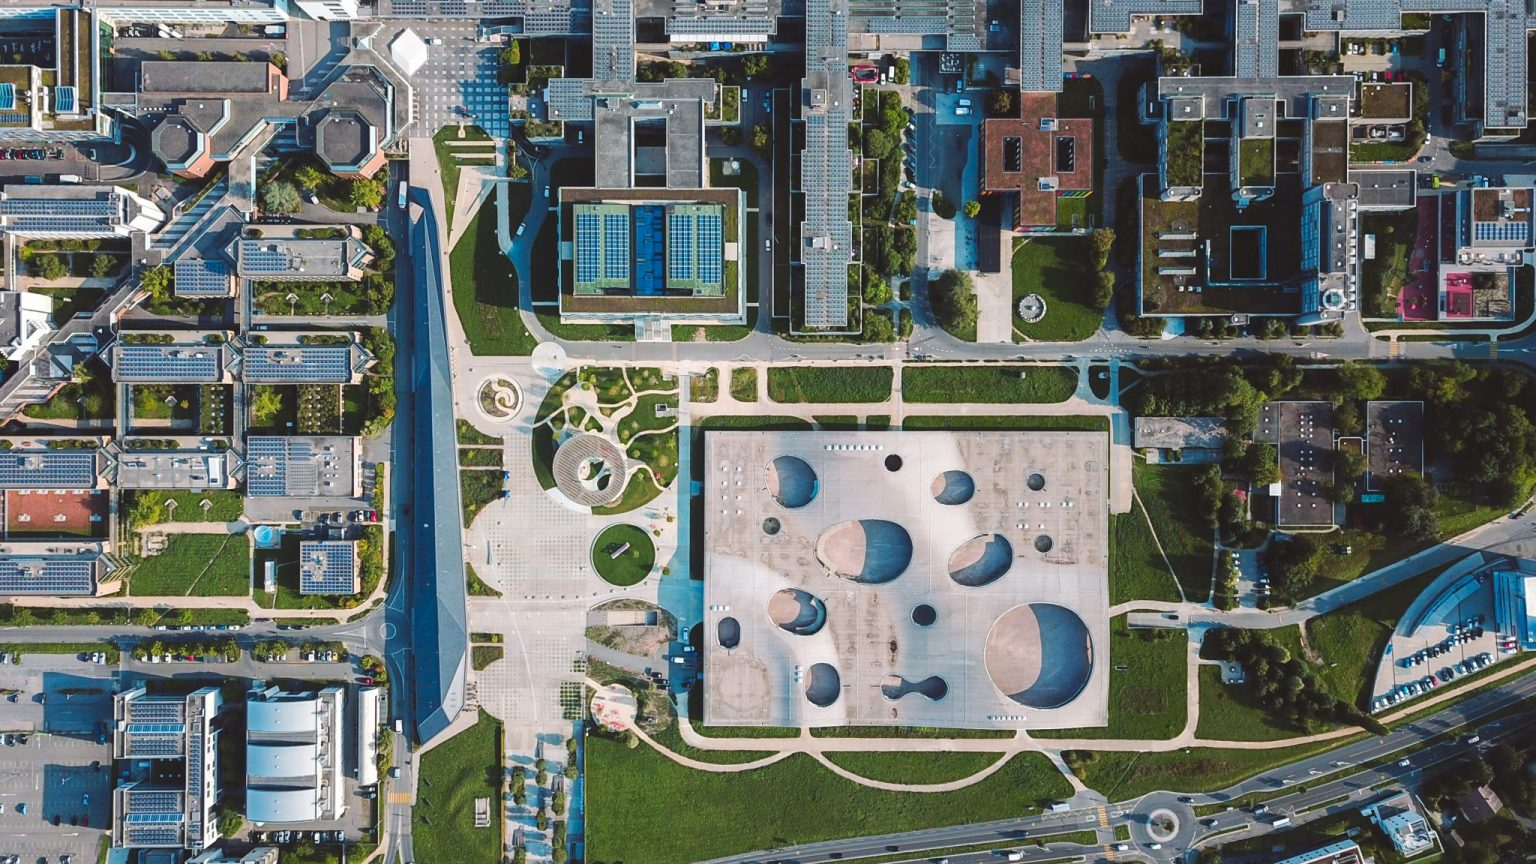
\includegraphics{figures/campus.jpg}
    \legende{Processus de sélection des modèles.}{Les modèles sont sélectionnées selon plusieurs critères : présence dans une des bases de données (GIEC, SCC, SSP, IAMC) ou dans une review. Ils sont ensuite comparés selon leurs caractéristiques.}
    \label{fig:méthodo-litrev}
\end{figure}

\section{Tour d'horizon des modèles et de leurs fonctions de dommage}

Les modèles intégrés sont très variés. Ils ont des histoires différentes (issus de l'énergie, de l'économie ou du climat), des perspectives différentes (en particulier entre les États-Unis ou l'Union européenne), des questions différentes, des choix de modélisation différents (simulation ou optimisation). 

\subsection{D'autres revues de littérature}

Revues de la littérature des différents modèles
\cite{diaz_quantifying_2017} => présente les trois SCC, les formes des fonctions de dommage et d'autres caractéristiques // c'est une base de mon travail puisque j'ai essaye de faire quelque chose d'assez similaire

\cite{souffron_successful_2024} => présente plein de modèles et les commente. Pas vraiment une revue de littérature sur les damage functions mais plus général, permet de bien se repérer dans la littérature + grosse emphase sur les modèles hétérodoxes

\cite{review of information on models}  Une revue des différents modèles 

Meta analyse des estimations du niveau du changement climatique
\cite{howard_few_2017} => 

\cite{gillingham_modeling_2018} gillingham => peut être à mettre dans la partie \ref{chapter:modelisation} ?

\cite{keppo_exploring_2021} => grosse revue de littérature sur les IAMs

\cite{harmsen_integrated_2021} => évaluation des IAMs à travers une méthodologie précise

\cite{krey_looking_2019} => comparaison des hypohtèses technologiques des modèles


Sur les types de modèles : 
\cite{mercure_modelling_2019} => présente les principales différences entre les modèles de simulation et d'optimisation, et montre que c'est aussi une différence paradigmatique. 
\subsection{Méthode : construction de la base de données}

\begin{table}[]
    \centering
    \begin{tabular}{c|c}
         &  \\
         & 
    \end{tabular}
    \legende{Les différents modèles recensés et leurs fonctions de dommage}{Description rapide}
    \label{tab:my_label}
\end{table}

\subsection{Premiers indicateurs quantitatifs}

\begin{figure}
    \centering
    %\includegraphics[width=0.5\linewidth]{}
    \legende{Visualisation graphique des différents modèles}{Description rapide}
    \label{fig:enter-label}
\end{figure}

\subsection{Les principaux modèles}

On présente ici rapidement des modèles, leurs caractéristiques générales et la forme de leur fonction de dommage. Il s'agit surtout de montrer la diversité des approches de modélisation, et non d'avoir un recensement systématique. Les lecteurs plus curieux trouveront plus de caractéristiques en suivant le lien. \blog{https://damage-functions-modeling.readthedocs.io/en/latest/1_introduction/functions.html}

\subsubsection{DICE}

DICE veut dire XXX et constitue une des premières tentatives de modéliser les relations entre l'économie et le climat. Il comporte une fonction de dommage, extremement simplifiée. 

\begin{equation}
\begin{array}{ll}
    & \displaystyle  \Delta = \psi_{1}T_{AT}(t) + \psi_{2}[T_{AT}(t)]^{2} \\
    & = [0.0]T_{AT}(t) + [0.003467][T_{AT}(t)]^{2}
\end{array}
\label{eq:df_dice2023}
\end{equation}

\subsubsection{FUND} 

A l'inverse, FUND présente un niveau de désagrégation assez avancé. Il y a de nombreuses fonctions de dommage, qui sont utilisées les unes dans les autres. Leur forme générale est d'obtenir un niveau de dommage à partir d'une elasticité entre un phénomène et un autre. 

Par exemple, l'impact du changement climatique sur l'agriculture est construit par la somme de trois canaux : d'une part, l'impact du niveau de changement climatique; d'autre part, la vitesse de ce changement (représenté en \ref{eq:fund_A2}); enfin, l'augmentation de la fertilisation des plantes. 

\begin{equation}
    A_{t,r}^{r}=\alpha_{r}\left(\frac{\Delta T_{t}}{0.04}\right)^{\beta}+\left(1-\frac{1}{\rho}\right)A_{t-1,r}^{r}
    \label{eq:fund_A2}
\end{equation}

D'autres impacts sont aussi représentés, tels que l'impact du niveau des eaux sur le littoral, les écosystèmes, les domages liés aux cyclones tropicaux et extra-tropicaux, etc. , et ce par différents biais : des dommages directs (monétaires), et la monétarisation de perte de vie ou de perte de temps de vie. 

\begin{equation}
    D_{t,r}^{\nu}=D_{1990,r}^{\nu}Q_{r}^{\nu}\left(T_{t}-T_{1990}\right)^{\beta}\left(\frac{y_{t,r}}{y_{1990,r}}\right)^{\gamma}
    \label{eq:fund_HV}
\end{equation}

\begin{equation}
    V S L_{t,r}=\alpha\left(\frac{y_{t,r}}{y_{0}}\right)^{\gamma}
    \label{eq:VSL}
\end{equation}

\subsubsection{Autres formes quadratiques}

Les formes quadratiques issues de DICE/RICE ont été grandement critiquées (voir section \ref{ss:forme}), et d'autres formes quadratiques sont apparues. C'est le cas notamment dans DEFINE (\ref{eq:DEFINE}), dont on peut trouver une forme très similaire dans le Giraud Stock-Flow consistent model. Il s'agit d'équations qui, comme DICE, sont extrememnt simplifiées et aggrégée, mais la forme de la relation est différente. 

\begin{equation}
    \Delta T = 1 - \frac{1}{1 + \eta_1 TAT + \eta_2 TAT^2 + \eta_3 TAT}
    \label{eq:DEFINE}
\end{equation}

\subsubsection{Autres formes non quadratiques}



\section{Trois questions centrales}


\subsection{La forme : comment représenter un phénomène qui n'existe pas encore ?}
\label{ss:forme}

La première difficulté quant à la représentation des impacts du changement climatique est le choix de la forme de la fonction de dommage. En effet, les phénomènes à l'origine des dommages climatiques sont à la fois incertains et récents. D'abord, les phénomènes physiques, dont on a du mal à avoir une représentation fiable et précise (voir notamment la section \ref{fig:tipping-point} sur les tipping points). Ensuite, et peut être plus encore, l'interaction entre ces évenements et les sociétés humaines est extremement difficile à comprendre, et donc à modéliser. Exercice de simplification, la modélisation nécessite pourtant d'extraire des lois générales de phénomènes particuliers, pour pouvoir établir des relations entre eux. \\

Ainsi, il est déjà très difficile de choisir une forme fonctionnelle qui soit adaptée. On peut contrer cet argument en avançant que la pratique de la modélisation doit assumer cette simplification. De ce point de vue, un modèle ne vise pas à reproduire la réalité ou des mécanismes réels, mais seulement à fournir un cadre explicatif suffisant pour rendre intelligible des choses qui ne l'étaient pas avant. \\

Le caractère récent des impacts du changement climatique, et encore plus de la prise en compte de ces effets en tant qu'effets du changement climatique, complique encore un peu la tâche. En effet, les séries temporelles étant courtes, il est difficile d'en extraire des formes fonctionnelles qui correspondraient effectivement à la relation entre les différentes variables. \\

Enfin, ces sources de données ne couvrent qu'un intervalle d'anomalie de température assez faible. En effet, on estime le réchauffement climatique actuel à environ 1.2 \textdegree C par rapport à la période pré-industrielle. Cependant, les estimations vont plus haut : l'accord de Paris pour le climat vise à avoir une réchauffement limité à 2 \textdegree C , et le plus proche possible de 1.5 \textdegree C; des estimations vont plus loin encore. Ainsi, des fonctions calibrées sur l'intervalle $[+0; +1.2]$ pourraient ne pas du tout capter les phénomènes observés dans le futur, sur un intervalle plus grand. Là réside un des grands défis de la modélisation des dommages : il s'agit de modéliser des phénomènes qui n'existent pas encore, et qui surviendront dans un contexte probablement très différent sur de nombreux aspects de celui dans lequel a lieu la modélisation. 

\begin{figure}[ht]
\centering
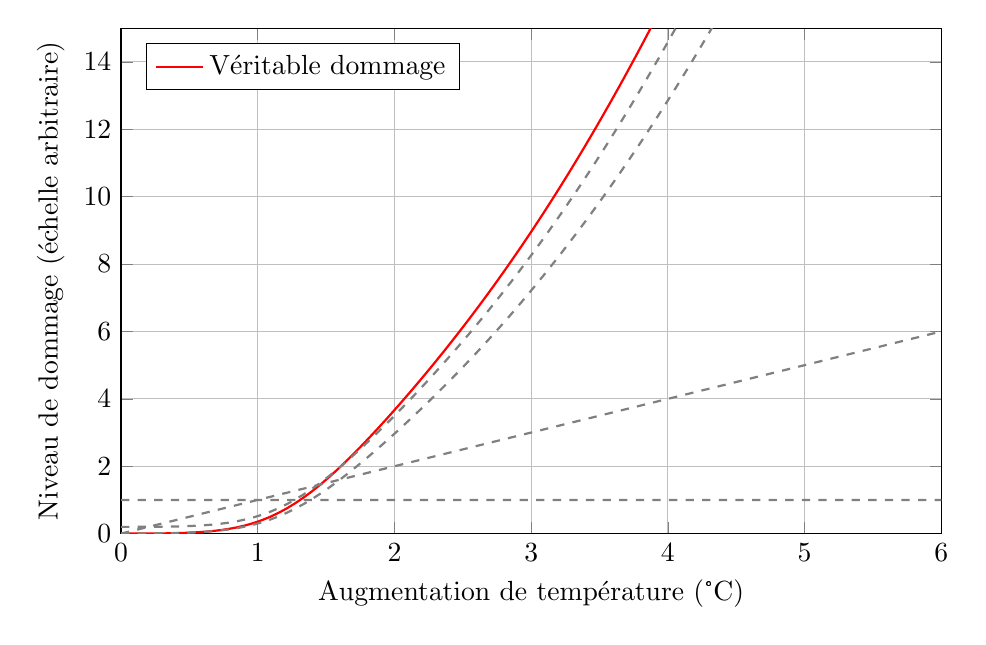
\begin{tikzpicture}
    \begin{axis}[
        width=12cm, height=8cm,
        xlabel={Augmentation de température (°C)},
        ylabel={Niveau de dommage (échelle arbitraire)},
        xmin=0, xmax=6,
        ymin=0, ymax=15,
        domain=0:6,
        legend pos=north west,
        samples=100,
        grid=major,
        legend cell align={left},
        every axis legend/.append style={nodes={right}}
    ]
    
    % Courbe principale (véritable) en rouge
    \addplot [thick, red] {x^2 / (1 + exp(3*(1.2-x)))};
    \addlegendentry{Véritable dommage}
    
    % Courbes incertaines (grises) avec différentes formes fonctionnelles
    \addplot [thick, gray, dashed] {0.8*x^2 / (1 + exp(3*(1.2-x))) + 0.3*sin(3*x)};
    \addplot [thick, gray, dashed] {x};
    \addplot [thick, gray, dashed] {cos(x)};
    \addplot [thick, gray, dashed] {0.9*x^2 / (1 + exp(3*(1.2-x))) + 0.2*cos(3*x)};
    
    % Ligne verticale à 1.2 degrés
    %\draw [dashed] (axis cs:1.2,0) -- (axis cs:1.2,15);
    %\node at (axis cs:1.4,14.5) [anchor=west] {1.2°C};

    \end{axis}
\end{tikzpicture}
\legende{Niveau de dommage en fonction de l'augmentation de température}{Différentes formes fonctionnelles peuvent avoir un pouvoir explicatif important sur l'intervalle $[+0; +1.2]$, sur lequel on dispose de données empiriques, tout en divergeant grandement pour des valeurs plus haute de changement de température. Une fonction de dommage correctement calibrée pour des phénomènes observés n'est pas forcément calibrée pour les phénomènes futurs.}
\end{figure}



\begin{figure}
    \centering
    %\includegraphics{}
    \legende{Analyse en composantes principales des modèles.}{Les modèles sont classés selon beaucoup de composantes, pour identifier des similitudes ou des patterns.}
    \label{fig:ACP}
\end{figure}

\subsection{Les paramètres : quel niveau de complexité faut-il, et que prendre en compte ?}

\begin{figure}
    \centering
    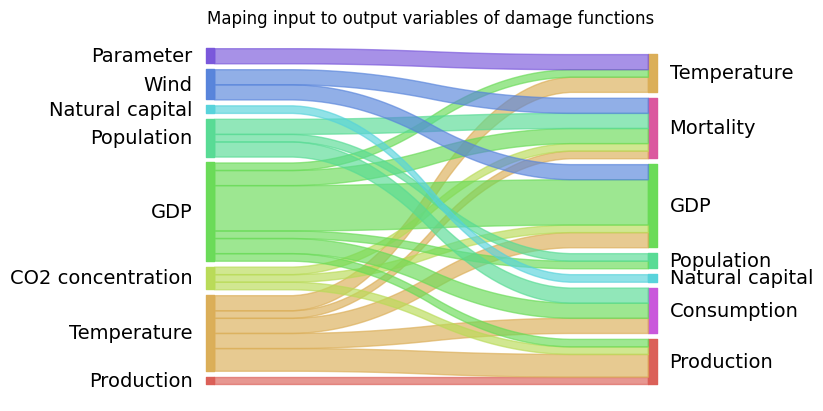
\includegraphics[width=0.9\linewidth]{figures/sankey.png}
    \legende{Sankey diagram des différentes fonctions}{Les modèles ne prennent pas en compte tous les mêmes données en entrées, et elles ne permettent pas d'expliquer les mêmes phénomènes.}
\end{figure}

\subsection{La calibration : un \textit{"tiens"} vaut-il deux \textit{"tu l'auras"} ?}

\section{Trois querelles pour répondre à ces questions}

\subsection{Le taux d'actualisation : la querelle Nordhaus / Stern}

\cite{guigourez_10_2023} => description de la querelle

\begin{figure}
    \centering
    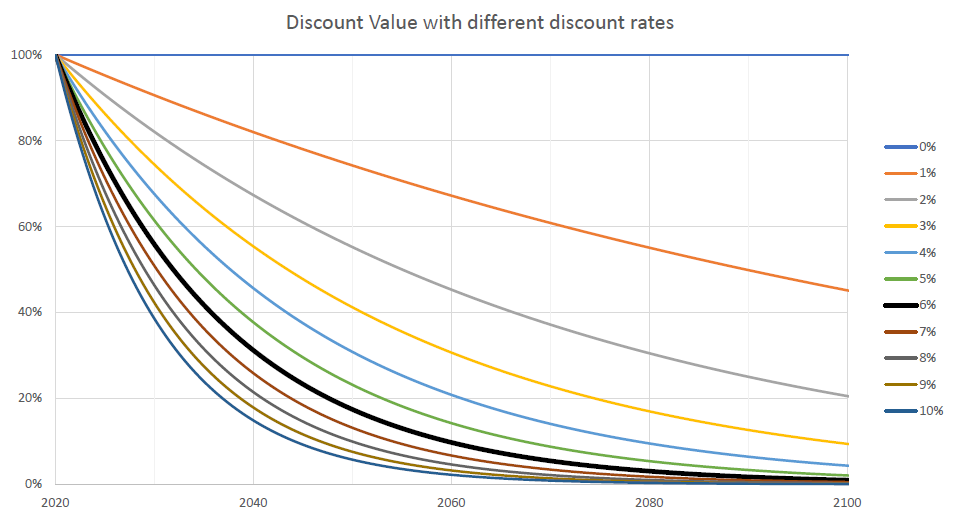
\includegraphics[width=\linewidth]{figures/actualisation.PNG}
    \legende{Valeur actualisée selon le temps et le taux d'actualisation}{Graphique qui représente la valeur d'une unité monétaire dans le temps, actualisée au présent, selon le taux d'actualisation. En jaune, celui choisi par Nordhaus, et en bleu celui choisi par Stern. Clé de lecture : avec un taux d'actualisation de 3\%, 100\$ de dommage en 2080 ne valent que 18\$ en 2020, alors que 100\$ de 2040 valent 56\$. }
    \label{fig:discount-rate}
\end{figure}

\subsection{Pourquoi représenter les dommages ? Les SCC vs le reste du monde}

Comme nous avons pu le voir, les critiques quant à la quantification et la monétarisation des dommages sont déjà nombreuses. Se pose donc la question suivante : faut-il représenter les dommages, et si oui, pourquoi et comment ? Pour éclairer ce dilemne, nous allons nous pencher sur deux une distinction particulière, entre les modèles qui représentent les dommages et ceux qui ne le font pas. \\

D'une part, certains modèles représentent des dommages de manière explicite. Ce sont essentiellement des modèles utilisés pour mesurer le coût social du carbone. Les arguments qui sont avancés par leurs défenseurs sont solides. Nous vivons dans un monde où la valorisation économique est centrale. Conformément à la théorie économique, et notamment à celle consacrée aux biens communs et aux externalités, si on ne peut pas compter la valeur de quelque chose, et surtout qu'elle ne s'impose pas à nous lors des transactions, alors cette valeur est invisible. De ce point de vue, et malgré les nombreuses limites (souvent assumées d'ailleurs) de la modélisation de ces phénomènes, il est nécessaire de représenter les dommages dans le modèle, même de manière imparfaite. En effet, selon ce point de vue, ne pas les représenter revient à les négliger, les omettre, ou en d'autre terme, à leur attribuer arbitrairement une valeur nulle. 
C'est dans cette perspective que se place de nombreux modèles, qui cherchent à proposer de nouvelles manières de représenter les dommages. Nombreux sont ceux qui, en réponse à la simplicité de la représentation de Nordhaus, ont proposé des fonctions de dommage toujours plus complexe, prenant en compte plus de mécanismes. 
\\

D'autre part, on peut argumenter que la représentation de ces dommages donne une fausse sensation de certitude. D'une part, elle done l'impression que le modèle est plus réaliste, en ce sens que ce qu'il dit \textit{serait} plus proche de la réalité et moins sujet aux travers de la simplification car justement plus complexe. Pourtant, on peut argumenter que la représentation des dommages, y compris quand elle est sophistiquée, fait appel à de nombreuses hypothèses, notamment concernant la permanence des phénomènes qui ont lieu. On a alors un modèle qui non seulement n'est pas forcément plus fiable ou plus proche de la réalité, mais qui est en plus nettement moins lisible, compréhensible - et dont les limites ne peuvent que très difficilement être interprétées et critiquées. 

\subsection{Compter ce qui n'a pas de prix : la difficile monétarisation}

